\chapter{Background}
\label{background}

\section{What is an electric dipole moment}

The most general description of an electric dipole moment (EDM) is as the centre of mass of a charge density distribution. This relationship can be expressed as

\begin{equation}
    \mathbf{d} = \int_V \rho(\mathbf{r}) \mathbf{r} dV
\end{equation}

where the EDM is denoted by $\mathbf{d}$ and the volume $V$ encloses the charge density distribution $\rho(\mathbf{r})$.

For a particle such as an electron one would typically expect this distribution to be symmetric, with a centre of charge at the centre of the object. However, as we will discuss shortly, an asymmetry is predicted in models of particle physics. Such an asymmetry in charge density for particles such as electron can be visualised as an egg-like shape, as shown in figure \ref{fig:electronEdmEgg}.

\begin{figure}[!htp]
  \centering
  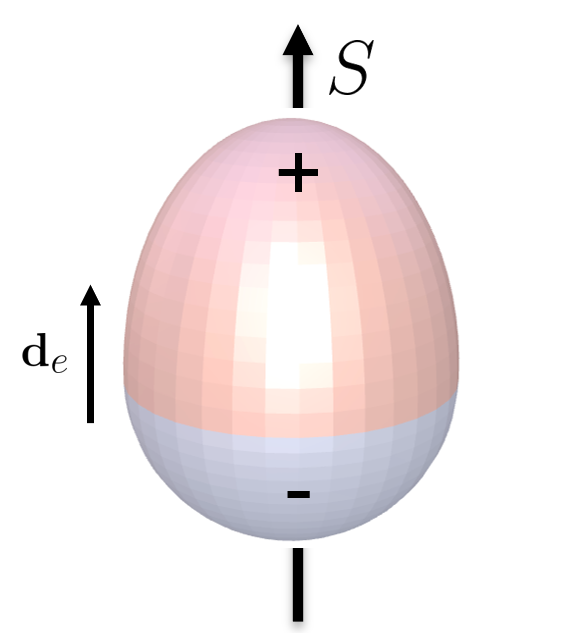
\includegraphics[scale=0.5]{images/EDM_egg.png}
  \caption{Illustration of an asymmetric charge distribution}
  \label{fig:electronEdmEgg}
\end{figure}

As the name suggests a key feature of an EDM is the moment on the dipole that results from an applied electric field. For such a dipole the non-relativistic Hamiltonian describing the interaction with an electric field is given by

\begin{equation} \label{dipole_energy}
    H_d = - \mathbf{d}_e \cdot \mathbf{E}.
\end{equation}

This Hamiltonian will be key to the interferometry used in the subsequently discussed experiments.

\section{Implications for fundamental theories}

There are two major challenges in attempts to explain our universe using the standard model: one is the apparent matter-antimatter imbalance of the universe and the other is apparent observations of dark matter. Many theories have been proposed to account for these unexplained observations, such as the theories of supersymmetry (SUSY) or the Multi-Higgs models, which introduce many symmetry violating particles, so far unobserved. However, before discussing these theories and their predictions, it is worth taking a brief detour in the history of symmetry violation.

\subsection{CPT Symmetry}

Prior to the 1950s it was believed that nature obeyed not only continuous symmetries but also discrete symmetries in charge, parity and time reversal. This view was challenged in 1956, with a review by Yang and Lee noting that whilst parity conservation had been demonstrated experimentally for strong and electromagnetic interactions, it had yet to be shown for weak interactions \cite{Lee_Yang_1956}. Shortly following the publication of this review parity was shown to be violated in the Wu experiment, in which beta decay was found to be favoured in the direction opposite to the nuclear spin \cite{Wu_1957}.

With parity symmetry experimentally violated, it was proposed that a combined charge-parity (CP) symmetry would still hold, however, this too was shown to be violated in the decay of neutral kaons in the 1960s \cite{Cronin_fitch_1964}. A proposed symmetry surviving these violations is a combined charge-parity-time (CPT) symmetry, which allows for CP symmetry violation under the requirement of a violation of T symmetry, a violation observed experimentally by the CPLEAR collaboration in 1998 \cite{CPLEAR_1998}.

The connection between the CPT theorem and particle EDMs arises from a particle EDM's inherent parity and time violation. In 1950 Purcell and Ramsay published an early discussion of the possibility for permanent EDMs of elementary particles such as the electron \cite{Purcell_Ramsay_1950}. In this discussion they showed that a non-zero particle EDMs would introduce an inherent violation of parity and time symmetry.

To understand this violation consider a particle with spin $\mathbf{S}$ and an EDM $\mathbf{d}_e$. From the special case of the Wigner-Eckart theorem applied to vector operators, known as the projection theorem, the dipole moment must lie along the axis of $\mathbf{S}$ \cite{Sakurai_1994}. A parity transformation would then result in $\mathbf{d}_e \rightarrow -\mathbf{d}_e$, with $\mathbf{S}$ remaining unchanged as $\mathbf{S}$ is pseudovector. On the other hand a time reversal transformation would result in  $\mathbf{S} \rightarrow -\mathbf{S}$ and $\mathbf{d}_e$ unchanged. These transformations are illustrated in figure \ref{fig:symmetry_violation}. In each of the two cases, a change in the relative orientations of the spin and EDM would result in different experimental results therefore creating a violation of parity and time reversal, since these violations occur in both parity and time the CPT theorem holds for particle EDMs.

\begin{figure}[!htp]
  \centering
  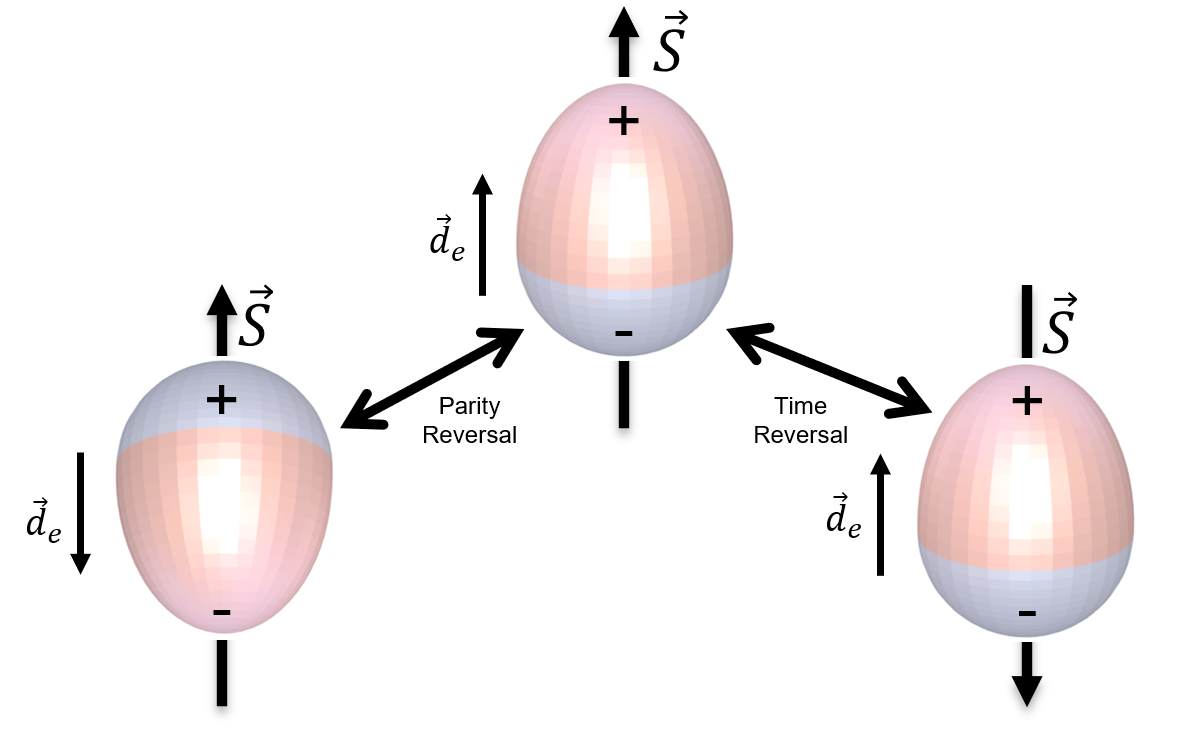
\includegraphics[scale=0.4]{images/symmetry_violation.png}
  \caption{Visualisation of the parity and time violation associated with a non-zero particle EDM. On the left a parity reversal transformation is shown, showing a change of sign in the particle's EDM, on the right a time reversal transformation is applied, resulting in the spin being flipped.}
  \label{fig:symmetry_violation}
\end{figure}

\subsection{Theoretical Predictions}

\begin{figure}[h]
    \centerline{
        \resizebox{12cm}{!}{
            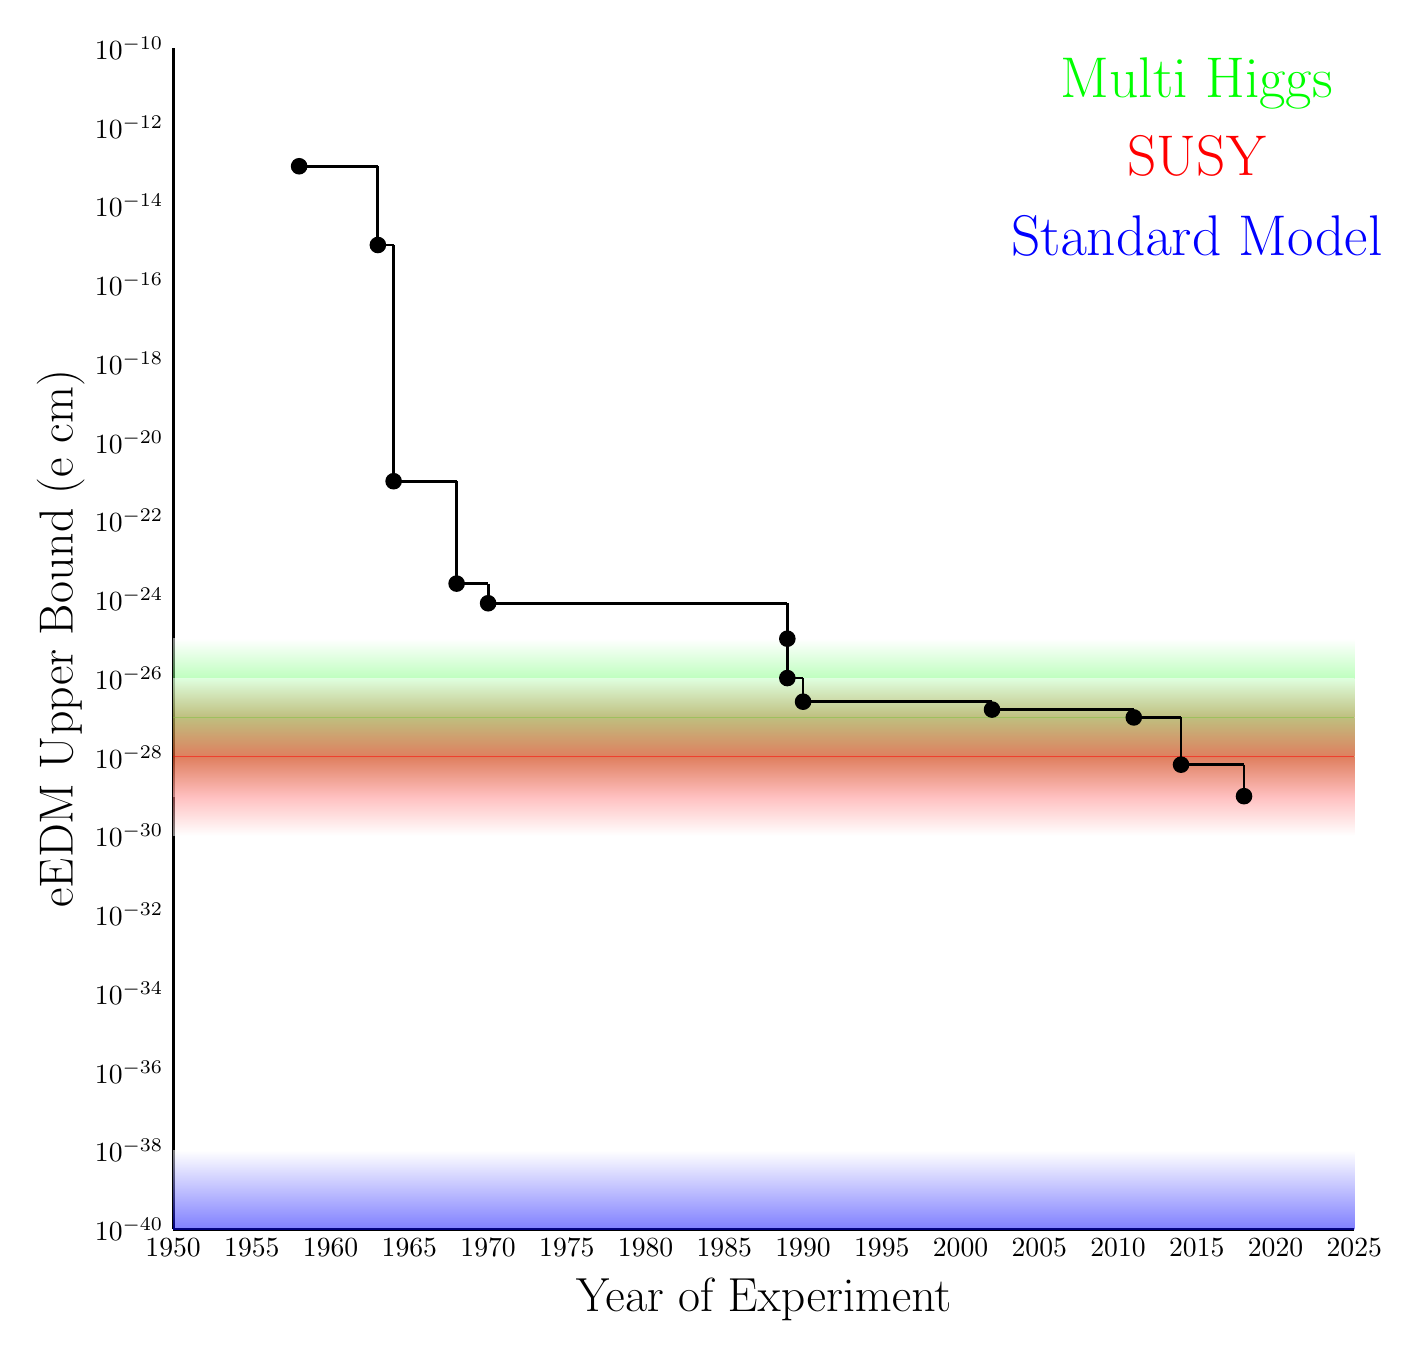
\begin{tikzpicture}
                \definecolor{laser}{RGB}{65,117,5}
                \definecolor{electric}{RGB}{208,2,27}
                \definecolor{magnetic}{RGB}{74,144,226}
                \definecolor{rf_boxes}{RGB}{155,155,155}
                
                \draw [line width=1pt]   (0,0) -- (0,15);
                \draw [line width=1pt]   (0,0) -- (15,0);
                
                \foreach \x [evaluate=\x as \y using {int(10 + 2 * \x)}] in {0,...,15}{
                    \node [anchor=east] at (0, 15 - \x) {$10^{-\y}$};
                }
                \node [anchor=east] at (-1, 7.5) {\rotatebox{90}{\LARGE eEDM Upper Bound (e cm)}};
                
                \foreach \x [evaluate=\x as \y using {int(1950 + 5 * \x)}] in {0,...,15}{
                    \node [anchor=north] at (0 + \x, 0) {$\y$};
                }
                \node [anchor=north] at (7.5, -0.5) {\LARGE Year of Experiment};
                
                \shade[bottom color=green, top color=white, opacity=0.5] (0,6.5) rectangle (15,7.5);
                \shade[bottom color=white, top color=green, opacity=0.5] (0,5.5) rectangle (15,6.5);
                \node [anchor=north, text=green] at (13, 15) {\huge Multi Higgs};
                
                \shade[bottom color=red, top color=white, opacity=0.5] (0,6) rectangle (15,7);
                \shade[bottom color=white, top color=red, opacity=0.5] (0,5) rectangle (15,6);
                \node [anchor=north, text=red] at (13, 14) {\huge SUSY};
                
                \shade[bottom color=blue, top color=white, opacity=0.5] (0,0) rectangle (15,1);
                \node [anchor=north, text=blue] at (13, 13) {\huge Standard Model};
                
                \fill (1.6, 13.5) circle[radius=3pt];
                \draw [line width=1pt]   (1.6, 13.5) -- (2.6, 13.5);
                \draw [line width=1pt]   (2.6, 13.5) -- (2.6, 12.5);
                \fill (2.6, 12.5) circle[radius=3pt];
                \draw [line width=1pt]   (2.6, 12.5) -- (2.8, 12.5);
                \draw [line width=1pt]   (2.8, 12.5) -- (2.8, 9.5);
                \fill (2.8, 9.5) circle[radius=3pt];
                \draw [line width=1pt]   (2.8, 9.5) -- (3.6, 9.5);
                \draw [line width=1pt]   (3.6, 9.5) -- (3.6, 8.2);
                \fill (3.6, 8.2) circle[radius=3pt];
                \draw [line width=1pt]   (3.6, 8.2) -- (4, 8.2);
                \draw [line width=1pt]   (4, 8.2) -- (4, 7.95);
                \fill (4, 7.95) circle[radius=3pt];
                \draw [line width=1pt]   (4, 7.95) -- (7.8, 7.95);
                \draw [line width=1pt]   (7.8, 7.95) -- (7.8, 7.5);
                \fill (7.8, 7.5) circle[radius=3pt];
                \draw [line width=1pt]   (7.8, 7.5) -- (7.8, 7);
                \draw [line width=1pt]   (7.8, 7) -- (7.8, 7);
                \fill (7.8, 7) circle[radius=3pt];
                \draw [line width=1pt]   (7.8, 7) -- (8, 7);
                \draw [line width=1pt]   (8, 7) -- (8, 6.7);
                \fill (8, 6.7) circle[radius=3pt];
                \draw [line width=1pt]   (8, 6.7) -- (10.4, 6.7);
                \draw [line width=1pt]   (10.4, 6.7) -- (10.4, 6.6);
                \fill (10.4, 6.6) circle[radius=3pt];
                \draw [line width=1pt]   (10.4, 6.6) -- (12.2, 6.6);
                \draw [line width=1pt]   (12.2, 6.6) -- (12.2, 6.5);
                \fill (12.2, 6.5) circle[radius=3pt];
                \draw [line width=1pt]   (12.2, 6.5) -- (12.8, 6.5);
                \draw [line width=1pt]   (12.8, 6.5) -- (12.8, 5.9);
                \fill (12.8, 5.9) circle[radius=3pt];
                \draw [line width=1pt]   (12.8, 5.9) -- (13.6, 5.9);
                \draw [line width=1pt]   (13.6, 5.9) -- (13.6, 5.5);
                \fill (13.6, 5.5) circle[radius=3pt];
                
            \end{tikzpicture}
            
            
        }
    }
    \caption{A graph of the experimental upper bounds placed on a possible eEDM, with the range of theoretical predictions from the Standard Model and several BSM theories overlayed \cite{Pendlebury_Hinds_2000}.}
    \label{fig:experimental_history}
\end{figure}

Since its development through the latter half of the $\text{20}^\text{th}$ century, the Standard Model of particle physics has proven highly accurate in its experimental predictions, notably in predictions of quarks, the tau neutrino and most recently the Higgs boson. A criticism however of the Standard Model is the limited CP violation it permits, a phenomenon thought to be a critical mechanism in accounting for phenomenon such as the observed matter-antimatter imbalance of the universe. This limited CP violation leads to the Standard Model predicting an incredibly small eEDM of typically $< 10^{-38}$ e cm \cite{Pospelov_2005}.

Deviating from the standard model are the various BSM (Beyond Standard Model) theories, such as the family of supersymmetric theories (SUSY). These theories have attempted to resolve issues with the Standard Model such as the hierachy problem\footnote{The hierachy problem addresses the large difference between the scales of various quantities in different fundamental forces, for example the masses of the W and Z particles (the force carriers of the weak force) are $10^{16}$ times smaller than than the Planck mass (the mass scale of gravity). An introduction to this problem can be found at \cite{Strassler_2011} and a more detailed discussion of application of of supersymmetry to the hierachy problem can be found in \cite{Stephen_1998}} via, in the case of supersymmetry, introducing a supersymmetry between bosons and fermions. This supersymmetry leads to a whole scheme of additional of superpartners to Standard Model particles, with the energies of the lightest of which thought to lie a few orders of magnitude above the TeV scale \cite{Stephen_1998}. Whilst many proponents of supersymmetry are hopeful of the detection of these superpartners at there LHC, it is proving very challenging to explore these TeV energy scales. An implication of these superpartners is greater CP violation, which relates to eEDM searches as it leads to greater predictions for the magnitude of an eEDM. For a detailed discussion of particle EDMs in supersymmetry please refer to Nakai et al \cite{Nakai_2017}.

This observation provides an alternative experimental test for these theories and their predicted superpartners, through measuring a non-zero eEDM with a magnitude greater than the $\sim 10^{-38}$ e cm upper bound of the Standard Model. With the recent progress in eEDM measurements, as well as the potential for significant improvement in the near future, this route is very promising.